\chapter{Neutrino Oscillations}
\label{ch:intro}

The study of neutrinos and their oscillations has been the source
of countless surprises in the development of the
Standard Model of particle physics and beyond.
Neutrinos are currently the only particles exhibiting properties
not explained by the Standard Model
which can be studied---not just searched for---on Earth in a laboratory setting.
This chapter will introduce the history of neutrinos (\cref{sec:history});
describe the modern theoretical understanding of neutrinos,
both in the Standard Model and beyond (\cref{sec:theory});
and present the experimental techniques used to study neutrino oscillations,
focusing on those used by the Daya Bay experiment (\cref{sec:experiment_intro}).


\section{History of neutrinos}
\label{sec:history}

The first evidence of neutrinos emerged in the form of
the continuous spectrum of $\beta$ particles
emitted during nuclear decay.
The continuous spectrum was first reported by Chadwick in 1914 \cite{chadwick_beta}.
Additional measurements confirming Chadwick's result accumulated over the next decade.
At the time, $\beta$ decay was thought to be a 2-body decay:
\begin{equation}\label{eq:old_beta}
    N(A, Z) \to N(A, Z+1) + \beta^-
\end{equation}
Conservation of energy uniquely determines the energy
of the outgoing $\beta$ particles for a given decay,
thus producing a monoenergetic spectrum,
as had been observed for $\alpha$ and $\gamma$ decays.
In 1931, rather than sacrifice the principle of conservation of energy,
Pauli proposed the introduction of a light neutral particle
produced during $\beta$ decay that escaped detection
due to a low interaction cross section \cite{pauli_letter}.
The particle, eventually named the neutrino ($\nu$) by Fermi,
provided the additional degree of freedom needed
to maintain conservation of energy and allow for a continuous $\beta$ spectrum
via the 3-body decay
\begin{equation}\label{eq:beta_mid}
    N(A, Z) \to N(A, Z+1) + \beta^- + \nu
\end{equation}
Subsequent experiments, detailed below,
would reveal the existence of an antineutrino $\bar{\nu}$,
followed by a distinction between neutrino flavors $\nu_e, \nu_\mu,$
and, much later, $\nu_\tau$.
Additionally, the discoveries of the proton and neutron
led to the conclusion that $\beta$ decay was the result of
the decay of a single neutron rather than of the nucleus as a whole.
The modern understanding of $\beta$ decay is therefore
\begin{equation}\label{eq:beta_modern}
    n \to p + e^- + \nuebar
\end{equation}
This process and its permutations
provide the vast majority of opportunities for
experimental investigation of the neutrino to this day.

\subsection{Discovery of the neutrino}
\label{subsec:discovery}

Reines and Cowan were the first to observe the neutrino experimentally in 1956
\cite{reines_cowan}.
They used a liquid scintillator detector to monitor a target of
water with dissolved $\text{CdCl}_2$
placed near the Savannah River Plant nuclear reactor.
The neutrinos were expected to undergo the inverse beta decay (IBD) reaction,
\begin{equation}\label{eq:ibd}
    \nuebar + p \to n + e^+,
\end{equation}
with the proton supplied by a hydrogen nucleus (\isotope[1]{H}) in the water.
The positron would annihilate in the water almost immediately,
producing two $\gamma$ rays which were detected in the liquid scintillator
as a prompt signal.
The neutron would scatter within the target for a few ($\sim5$) \si{\us}
and eventually capture on a Cd nucleus,
triggering the emission of several $\gamma$ rays totalling \SI{9}{\MeV},
detected as a delayed event by the liquid scintillator.
IBD events were identified by the coincidence of a prompt and delayed event
at a rate of \SI[per-mode=reciprocal]{2.88\pm0.22}{\per\hour},
only present when the reactor was powered on.
This experiment was the progenitor of the Daya Bay experiment,
which also observes IBD events using a liquid scintillator detector
and the principle of the prompt-delayed coincidence.

\subsection{Difference between \texorpdfstring{$\nu$ and $\bar{\nu}$}{nu and nu-bar}}
\label{subsec:nu_vs_nubar}

Even prior to Reines and Cowan's observation of the neutrino,
Davis was able to provide convincing evidence that
the antineutrino was different from the neutrino \cite{davis_diff_nuebar}.
In 1954, Davis attempted to observe the reaction
\begin{equation}\label{eq:davis_nubar}
    \isotope[37]{Cl} + \bar{\nu} \to \isotope[37]{Ar} + \beta^-
\end{equation}
which is forbidden by lepton number conservation.
If $\nu=\bar{\nu}$, then lepton number conservation is violated
and the reaction could occur.
A tank containing \SI{3900}{\liter} of $\text{CCl}_4$
was placed in close proximity to the Brookhaven nuclear reactor.
Any \isotope[37]{Ar} produced was extracted using helium gas,
and the resulting gas was monitored using a Geiger counter
to observe the decay of \isotope[37]{Ar} (half-life 35 days).
No additional decays of \isotope[37]{Ar} were observed over the background rate.
Thus it was concluded that $\nu\neq\bar{\nu}$.

Davis noted in the conclusion of his report that the same experimental setup
could be used to detect neutrinos produced by the sun.
This experiment will be discussed later as the earliest evidence
for neutrino oscillations.

\subsection{Helicity of the neutrino}
\label{subsec:helicity}

The helicity $\frac{\sigma\cdot p}{\vert p\vert}$ of the neutrino was measured by
Goldhaber, Grodzins and Sunyar in 1957 \cite{helicity_measurement,helicity_review}.
The reaction chain
\begin{align}\label{eq:lampshade}
    \begin{split}
        e^- + \isotope[152m]{Eu}(0^-) \to \nu_e
        + & \isotope[152]{Sm}^*(1^-) \\
          & \isotope[152]{Sm}^*(1^-) \to \isotope[152]{Sm}(0^+) + \gamma
    \end{split}
\end{align}
allows for a connection between the helicity (polarization)
of the emitted $\gamma$
with the helicity of the $\nu_e$, which is not directly detected,
as follows.
The total inital momentum is approximately 0.
Therefore the decay products $\nu_e$ and $\isotope[152]{Sm}^*(1^-)$
must have equal and opposite momenta.
Similarly, the initial angular momentum (including spin) is $\pm\nicefrac{1}{2}$,
and the daughter nucleus is known to have spin 1,
therefore the spins of the decay products must point in opposite directions.
Since both decay products have spins and momenta in opposite directions,
they must have the same helicity.
When the $\isotope[152]{Sm}^*(1^-)$ decays,
occasionally the $\gamma$ will be emitted in the same direction
as the momentum of the parent nucleus (recoiling against the $\nu_e$).
In this case, since the final state of the \isotope[152]{Sm} has spin 0,
the $\gamma$ must have the same spin and direction of momentum
as the parent $\isotope[152]{Sm}^*$ and therefore the same helicity as the $\nu_e$.
If the $\gamma$ is emitted in a different direction,
it has a nonzero probability of having the opposite helicity.
A method was required to select only those $\gamma$ rays which
were emitted in the same direction as the momentum of the parent nucleus
to ensure they had the same helicity as the emitted $\nu_e$.

\begin{figure}
    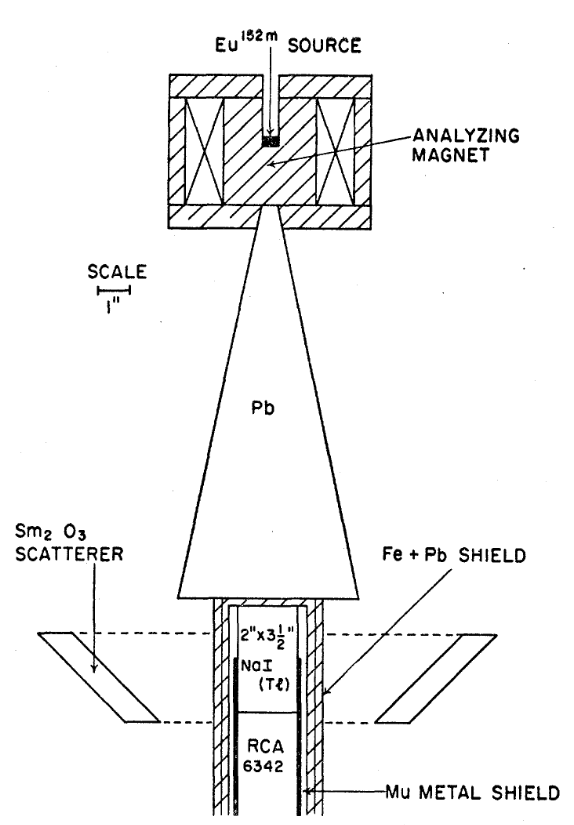
\includegraphics[width=0.5\textwidth]{ch_introduction/helicity_setup}
    \caption{
        Schematic layout of the experiment which measured
        the helicity of the neutrino \cite{helicity_measurement}.
    }
    \label{fig:lampshade}
\end{figure}

A solution was found in the form of resonant fluorescence,
the absorption and re-emission of a $\gamma$ ray
by a nucleus with an energy level equal to that of the $\gamma$ ray.
An obvious choice for this setup was the exact same isotope of $\isotope[152]{Sm}$,
so target of $\text{Sm}_2\text{O}_3$
containing \SI{26.8}{\percent} \isotope[152]{Sm}
was placed in a ring below the sample of \isotope[152]{Eu}
(\cref{fig:lampshade}).
The $\gamma$ rays which resonantly scattered on the $\text{Sm}_2\text{O}_3$
were detected using a NaI scintillation counter.
This arrangement selected only the desired $\gamma$ rays
(those emitted in the same direction as the parent nucleus)
due to the following properties of resonant fluorescence:
The emitted $\gamma$ rays are in general
slightly (\SI{\sim3}{\eV}) below the energy
needed to re-excite the same mode in a target nucleus
due to the recoil during absorption.
The $\gamma$ rays emitted in exactly the same direction
as the parent $\isotope[152]{Sm}^*$
experince a recoil on emission which takes the form of
a Doppler shift to higher energy
(due to the parent's own recoil against the $\nu_e$).
Even the additional energy from the maximal Doppler shift
was not sufficient to cause the resonant fluorescence;
only when coupled with the random thermal motion
of both the parent and target nuclei
was there a non-negligible probability of interaction.
Thus the $\gamma$ rays reaching the NaI counter
must have been resonantly scattered off the target \isotope[152]{Sm};
therefore they must have been emitted in exactly the same direction
as the parent $\isotope[152]{Sm}^*(1-)$,
carrying the same helicity as the $\nu_e$
that caused the initial recoil.

The helicity of the emitted $\gamma$ rays was measured
using an electromagnet surrounding the \isotope[152]{Eu} source.
When the electrons in the magnet were polarized in a particular direction,
only $\gamma$ rays with the opposite polarization (spin)
would Compton scatter off them.
By comparing the number of resonant scatters
using an upward-pointing magnetic field
with the number from a downward-pointing field,
the polarization, and therefore the helicity, could be measured.
With the field pointing up, the polarized electron spins point down,
and therefore a downward-traveling $\gamma$ ray
would only scatter if it had a upward-pointing spin, i.e. helicity $-1$.
Conversely, downward-traveling $\gamma$ rays
with helicity $-1$ are preferentially transmitted
when the field is pointing down.
Only the transmitted $\gamma$ rays have the opportunity to
resonantly scatter off the $\text{Sm}_2\text{O}_3$
and be detected by the NaI counter.
A measured excess of
$\frac{2(N_{\downarrow}-N_{\uparrow})}{N_{\downarrow}+N_{\uparrow}} =
\num{0.017\pm0.003}$
was observed,
indicating that the $\gamma$ rays, and therefore the neutrino,
had helicity $-1$.


\subsection{Discovery of neutrino flavors}
\label{subsec:nu_flavors}

In 1962, Schwartz, Lederman and others used the
Alternating Gradient Synchrotron (AGS) at Brookhaven
to demonstrate that $\nu_\mu$ behaved differently from $\nu_e$
\cite{numu_vs_nue}.
In the world's first accelerator neutrino experiment,
they produced a beam of $\nu_\mu$ by directing
the \SI{15}{\GeV} AGS proton beam
onto a fixed beryllium target and relying on the following reaction chain:
\begin{align}\label{eq:accel_reaction_chain}
    \begin{split}
        p + \text{Be} \to &\pi^{\pm} + X \\
        &\pi^{\pm} \to \mu^{\pm} + \nu(\bar{\nu}) \\
    \end{split}
\end{align}
A series of spark chambers of total target mass \SI{10}{\tonne}
was exposed to the neutrino beam,
with the non-neutrino beam products attenuated
by a \SI{13.5}{\m} thick steel wall.
In a universe with only one type of neutrino (and one type of antineutrino),
then the neutrino beam would have produced equal quantities
of electrons and muons.
After an exposure of \num{3.48e17}~protons ($\sim300$~hours),
a total of 113 events were observed,
of which 56 were identified as muon-like single-track or vertex events
(5 of which were statistically attributed to cosmic ray contamination),
8 were electron-like electromagnetic showers, and 49 were background.
The electron-like events were attributed to
kaon contamination in the beam,
and, in any event, were not consistent with the
expected energy distribution of events due to the
primary muon-associated neutrino beam.
With dozens of muon events and not a single electron event
attributable to the muon-associated neutrinos,
it was concluded that $\nu_\mu \neq \nu_e$.


\subsection{Discovery of the neutral current}
\label{subsec:neutral_current}

In 1973, the Gargamelle neutrino experiment at CERN
published an observation of neutrino interactions
that did not involve a charged lepton,
thus proving the existence of the hadronic neutral current (NC) weak interaction
\cite{gargamelle_short,gargamelle}.
The Gargamelle bubble chamber contained \SI{\sim10}{\tonne} of
$\text{CF}_3\text{Br}$ within a \SI{2}{\tesla} magnetic field.
It was exposed to a neutrino beam which could switch
between $\nu_\mu$ and $\bar{\nu}_\mu$ modes.
A search was undertaken for events of the form
\begin{align}\label{eq:neutral_current}
    \begin{split}
        \nu_\mu(\bar{\nu}_\mu) + \text{N} &\to \nu_\mu(\bar{\nu}_\mu)
        + \text{hadrons, and} \\
        \nu_\mu(\bar{\nu}_\mu) + \text{N} &\to \mu^-(\mu^+) + \text{hadrons},
    \end{split}
\end{align}
with the former representing NC interactions
and the latter representing charged current (CC).
102 $\nu$- and 64 $\bar{\nu}$-induced interactions were observed
with the NC signature of only hadrons as interaction products,
and no associated $\mu$.

Gargamelle also observed a small number of leptonic NC interactions
of the form $\nu + e \to \nu + e$.
The first such event observed was found by a graduate student
in 1974.
Example bubble chamber photographs of hadronic
and leptonic NC interactions are shown in \cref{fig:gargamelle}.

\begin{figure}
    \centering
    \begin{subfigure}{0.49\textwidth}
        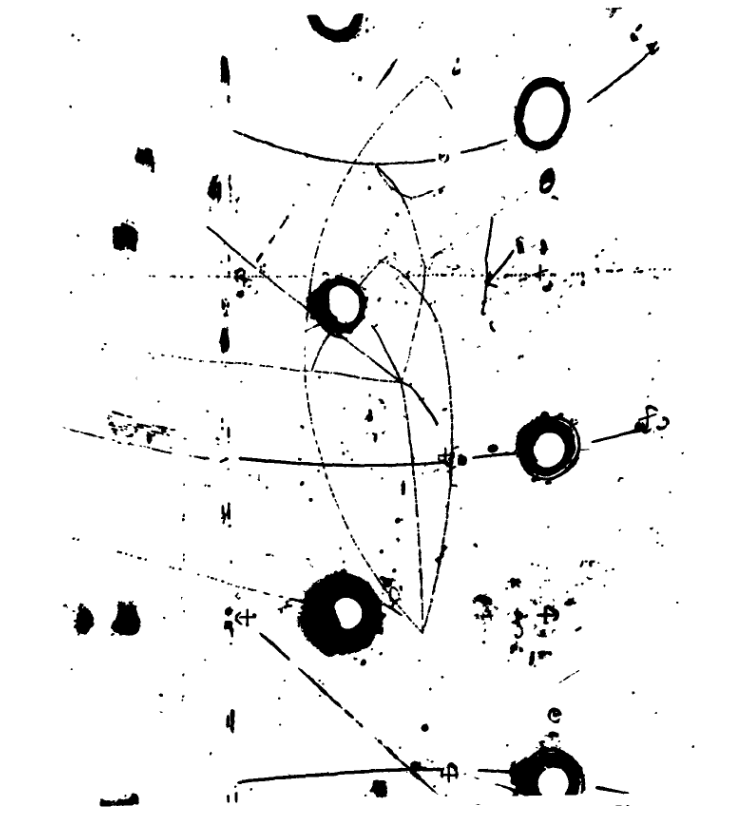
\includegraphics[width=\textwidth]{ch_introduction/gargamelle_hadronic}
    \end{subfigure}
    \begin{subfigure}{0.49\textwidth}
        \includegraphics[width=\textwidth]{ch_introduction/gargamelle_leptonic}
    \end{subfigure}
    \caption{
        Photographs of a hadronic NC interaction (left, \cite{gargamelle_leptonic})
        and the first observed leptonic NC interaction (right, \cite{gargamelle})
        taken by the Gargamelle neutrino experiment.
    }
    \label{fig:gargamelle}
\end{figure}


\section{Neutrinos in the Standard Model}
\label{sec:theory}

\section{Reactor neutrino experiments}
\label{sec:experiment_intro}

